% Options for packages loaded elsewhere
\PassOptionsToPackage{unicode}{hyperref}
\PassOptionsToPackage{hyphens}{url}
\PassOptionsToPackage{dvipsnames,svgnames*,x11names*}{xcolor}
%
\documentclass[
]{article}
\usepackage{amsmath,amssymb}
\usepackage{lmodern}
\usepackage{ifxetex,ifluatex}
\ifnum 0\ifxetex 1\fi\ifluatex 1\fi=0 % if pdftex
  \usepackage[T1]{fontenc}
  \usepackage[utf8]{inputenc}
  \usepackage{textcomp} % provide euro and other symbols
\else % if luatex or xetex
  \usepackage{unicode-math}
  \defaultfontfeatures{Scale=MatchLowercase}
  \defaultfontfeatures[\rmfamily]{Ligatures=TeX,Scale=1}
\fi
% Use upquote if available, for straight quotes in verbatim environments
\IfFileExists{upquote.sty}{\usepackage{upquote}}{}
\IfFileExists{microtype.sty}{% use microtype if available
  \usepackage[]{microtype}
  \UseMicrotypeSet[protrusion]{basicmath} % disable protrusion for tt fonts
}{}
\makeatletter
\@ifundefined{KOMAClassName}{% if non-KOMA class
  \IfFileExists{parskip.sty}{%
    \usepackage{parskip}
  }{% else
    \setlength{\parindent}{0pt}
    \setlength{\parskip}{6pt plus 2pt minus 1pt}}
}{% if KOMA class
  \KOMAoptions{parskip=half}}
\makeatother
\usepackage{xcolor}
\IfFileExists{xurl.sty}{\usepackage{xurl}}{} % add URL line breaks if available
\IfFileExists{bookmark.sty}{\usepackage{bookmark}}{\usepackage{hyperref}}
\hypersetup{
  pdftitle={Towards a robust desicion tool for ecosystems services in the industrial systems: A case study of Distributed recycling for additive manufacturing},
  colorlinks=true,
  linkcolor=blue,
  filecolor=Maroon,
  citecolor=Blue,
  urlcolor=Blue,
  pdfcreator={LaTeX via pandoc}}
\urlstyle{same} % disable monospaced font for URLs
\usepackage[margin=1in]{geometry}
\usepackage{longtable,booktabs,array}
\usepackage{calc} % for calculating minipage widths
% Correct order of tables after \paragraph or \subparagraph
\usepackage{etoolbox}
\makeatletter
\patchcmd\longtable{\par}{\if@noskipsec\mbox{}\fi\par}{}{}
\makeatother
% Allow footnotes in longtable head/foot
\IfFileExists{footnotehyper.sty}{\usepackage{footnotehyper}}{\usepackage{footnote}}
\makesavenoteenv{longtable}
\usepackage{graphicx}
\makeatletter
\def\maxwidth{\ifdim\Gin@nat@width>\linewidth\linewidth\else\Gin@nat@width\fi}
\def\maxheight{\ifdim\Gin@nat@height>\textheight\textheight\else\Gin@nat@height\fi}
\makeatother
% Scale images if necessary, so that they will not overflow the page
% margins by default, and it is still possible to overwrite the defaults
% using explicit options in \includegraphics[width, height, ...]{}
\setkeys{Gin}{width=\maxwidth,height=\maxheight,keepaspectratio}
% Set default figure placement to htbp
\makeatletter
\def\fps@figure{htbp}
\makeatother
\setlength{\emergencystretch}{3em} % prevent overfull lines
\providecommand{\tightlist}{%
  \setlength{\itemsep}{0pt}\setlength{\parskip}{0pt}}
\setcounter{secnumdepth}{5}
\usepackage{float}
\usepackage{subfig}
\usepackage[utf8]{inputenc}
\def\tightlist{}
\usepackage[bitstream-charter]{mathdesign}
\usepackage{pdflscape}
\usepackage{svg}
\usepackage{lineno}
\usepackage{setspace}
\newcommand*{\doverline}[1]{\overline{\overline{#1}}}
\usepackage{tabu}

\usepackage{multirow}
\usepackage{multicol}
\usepackage{colortbl}
\usepackage{hhline}
\usepackage{longtable}
\usepackage{array}
\usepackage{hyperref}
\ifluatex
  \usepackage{selnolig}  % disable illegal ligatures
\fi
\newlength{\cslhangindent}
\setlength{\cslhangindent}{1.5em}
\newlength{\csllabelwidth}
\setlength{\csllabelwidth}{3em}
\newenvironment{CSLReferences}[2] % #1 hanging-ident, #2 entry spacing
 {% don't indent paragraphs
  \setlength{\parindent}{0pt}
  % turn on hanging indent if param 1 is 1
  \ifodd #1 \everypar{\setlength{\hangindent}{\cslhangindent}}\ignorespaces\fi
  % set entry spacing
  \ifnum #2 > 0
  \setlength{\parskip}{#2\baselineskip}
  \fi
 }%
 {}
\usepackage{calc}
\newcommand{\CSLBlock}[1]{#1\hfill\break}
\newcommand{\CSLLeftMargin}[1]{\parbox[t]{\csllabelwidth}{#1}}
\newcommand{\CSLRightInline}[1]{\parbox[t]{\linewidth - \csllabelwidth}{#1}\break}
\newcommand{\CSLIndent}[1]{\hspace{\cslhangindent}#1}

\title{Towards a robust desicion tool for ecosystems services in the industrial systems: A case study of Distributed recycling for additive manufacturing}
\author{}
\date{\vspace{-2.5em}}

\begin{document}
\maketitle
\begin{abstract}
Ecosystem services (ES) is a powerful conceptual framework to put in evidence the benefits that humans received from nature, most of time for free.
The problem is that it is complex to link between the local ecosystem services of an urban territory and the industrial systems placed within it identifying the priority interactions (as synergy and impacts).
From a decision-maker perspective, there is no a aid decision tool to guide a multicriteria evaluation at early development stages of industrial systems.
There have been major efforts in the valuation of ES given by ecosystems (terrestrial, aquatic, atmospheric) to the human well-being (\protect\hyperlink{ref-Costanza2017}{Costanza et al. 2017}, \protect\hyperlink{ref-Costanza1997}{1997}; \protect\hyperlink{ref-DeGroot2012}{Groot et al. 2012}; \protect\hyperlink{ref-MEA2005}{MEA 2005}), and great advances in the developing of a standard ES baselines such as Common International Classification of Ecosystem Services (CICES)(\protect\hyperlink{ref-RoyHaines-Young2018}{Roy Haines-Young and Potschin 2018}).
However, few researches have been addressed the alignment the territorial priorities in terms of ES for planning and urban development with the supply/demand of ES by industrial systems.
In the industrial side, Life cycle thinking have been a major assessment tool putting a great attention in the quantification of the environmental impact of industrial interventions, and helping in the comparison of different scenarios in each aspect stage of the product life (\protect\hyperlink{ref-Mahmud2021}{Mahmud et al. 2021}; \protect\hyperlink{ref-Pryshlakivsky2021}{Pryshlakivsky and Searcy 2021}).
Recently, several research efforts reported accounts for the dependence systems by explicitly accounting for the demand that technological systems place on ecosystems and the supply of ecosystem services that nature can provide to a process or product at multiple spatial scales (\protect\hyperlink{ref-Liu2019g}{Liu and Bakshi 2019}).
This techno-ecological synergy (TES) (\protect\hyperlink{ref-Liu2019g}{Liu and Bakshi 2019}; \protect\hyperlink{ref-Bakshi2015}{Bakshi, Ziv, and Lepech 2015}) to reflect its emphasis on establishing mutually beneficial or synergistic relationships between technological and ecological systems, with the ultimate goal of achieving harmony between human activities and nature.
The purpose of this article is to propose a methodological approach in order to include ecosystem services in regarding the territorial and industrial endeavors.
This prioritization is based on the connection of urban ES services and the techno-ecological synergy.
The results of are step forwards to create techno-ecological synergies between ecological and industrial systems.
This methodological steps will applied to the case of distributed recycling via additive manufacturing (DRAM) to highlight the relevant ES from the CICES framework of this industrial system for the territory of Nancy, France.
The technical advancements of recycling approaches using additive manufacturing are promising technical interventions to foster plastic recycling at a local level.
\end{abstract}

{
\hypersetup{linkcolor=}
\setcounter{tocdepth}{2}
\tableofcontents
}
\linenumbers

\hypertarget{introduction}{%
\section{Introduction}\label{introduction}}

The current ecological urgency confirms that the understanding and managing the interactions between humans systems and the rest of nature is a major prerequisite for addressing the worsening environmental and social crises of the \(21^{st}\) century (\protect\hyperlink{ref-Lomborg2020}{Lomborg 2020}).
Even though engineering products and processes might meet the needs of the present, many of the technological developments are compromising the ability of future generations to meet their own needs (\protect\hyperlink{ref-ref}{\textbf{ref?}}).
For claiming for sustainability in technological development and interventions, the human activities should not exceed critical ecosystem capacity (\protect\hyperlink{ref-Bakshi2018}{Bakshi, Gutowski, and Sekulic 2018}).
This meta-principle is a imperative but not sufficient condition for sustainability.
Moreover, no country currently meets minimum thresholds for social development without exceeding planetary boundaries (\protect\hyperlink{ref-ONeill2018}{O'Neill et al. 2018}).
Therefore, it is no possible to rely only on techno-centric interventions without considering the finite planetary ecosystem characterized by profound uncertainty and the shared goals of ecological sustainability and just distribution (\protect\hyperlink{ref-ref}{\textbf{ref?}}).
We need to integrate ecological carrying capacity since the fuzzy front end phase of an industrial systems.
However, the integration of ecological aspects in the decision-making seems not evident given the complexity to define the boundaries and interactions of industrial and ecological systems.

\protect\hyperlink{ref-Ceschin2016}{Ceschin and Gaziulusoy} (\protect\hyperlink{ref-Ceschin2016}{2016}) putted forward the evolution of \emph{Design for Sustainability (DfS)} framework showing the different approaches that have evolved from a product innovation level to socio-technical systems level.
They pointed out that engineering interventions at only technological unit operation/product level are necessary, but not sufficient condition for sustainability.

The economic valuation of ecosystem goods and services gives an elegant framework highlighting their importance for society and human welfare.
However, there is a need to explicitly account for their contribution when designing and developing products and services (\protect\hyperlink{ref-Diwekar2021}{Diwekar et al. 2021}).
The engineering discipline developed the implicit assumption that ecological systems have nearly endless capacity to provide resources and adsorb wastes.
This blindness in the engineering vision can be explaining by the fact that at the beginning of the technological industrialization, the human activites' impacts on the earth remained marginal. This scenario is not true today.
The need for ecosystem services research has become evident due to the impacts of population growth, economic activities, and urbanization on natural capital (\protect\hyperlink{ref-Torres2021}{Torres, Tiwari, and Atkinson 2021}).
The loss in value associated with biodiversity loss and the related loss of ecosystem services is often invisible and does not influence decision makers (\protect\hyperlink{ref-Bruel2018}{Bruel et al. 2019}).
It is difficult to provide information about pressure from industrial systems in corporate information systems.
Engineering within ecological constraints need to acknowledge the capacity of relevant ecosystems to supply the demanded goods and services while the ecosystems and natural capital must be protected, restored and developed to be capable of continuing to supply those services that industry (and society) relies on (\protect\hyperlink{ref-Bakshi2018}{Bakshi, Gutowski, and Sekulic 2018}).

According to the Milleniums 15 out of 24 ecosystems services examined are degraded or being used in an unsustainable manner (\protect\hyperlink{ref-MEA2005}{MEA 2005}).
Likewise, using the planetary boundaries framework, it is argued that anthropogenic activities already exceed the biophysical limits of the ``safe operating zone'' in terms of carbon and nitrogen cycles, and biodiversity loss (\protect\hyperlink{ref-Rockstrom2009}{Rockström et al. 2009}; \protect\hyperlink{ref-ONeill2018}{O'Neill et al. 2018}).
Among the root causes of ecological degradation is ignorance about the exceed of the ecological carrying capacity in many decisions (\protect\hyperlink{ref-Liu2019g}{Liu and Bakshi 2019}; \protect\hyperlink{ref-Rodrigues2021}{Rodrigues et al. 2021}).
Another crucial issue is that current design approaches based on life cycle characterization and footprint methods focus on continuous improvement by reducing life cycle impacts per unit of product, encouraging improvements by doing ``less bad,'' which need not translate into keeping human activities within ecological constraints.
Ideally, it is needed to (re)designed industrial activities to reduce the demand for the demand of ecosystems services creating for a local `\emph{island of sustainability}' (\protect\hyperlink{ref-Wallner1996}{Wallner, Narodoslawsky, and Moser 1996}) which is that the demand should not exceed the supply at the local scale (\protect\hyperlink{ref-Gopalakrishnan2016}{Gopalakrishnan, Bakshi, and Ziv 2016}).
Therefore, it's urgent to expand the boundaries for engineering design from the lowest molecular level to the process level, and from individual process to the higher levels of value chains, ecosystems and the planet (\protect\hyperlink{ref-Martinez-Hernandez2017}{Martinez-Hernandez 2017}).

\protect\hyperlink{ref-Bakshi2015}{Bakshi, Ziv, and Lepech} (\protect\hyperlink{ref-Bakshi2015}{2015}) reported a framework of Techno-Ecological Synergy (TES) in order to expand the scope of the usual techno-centric perspectives.
The main point argued is that TES develops ways of enhancing synergies between a local scale manufacturing process and the land around it.
The final aims is to encourage a more robust analysis of technological and ecological systems at multiple spatial scales ranging from local (e.g.~for small systems such as a house and its yard, a manufacturing process and its site) to a larger scale systems that extend to consider the entire life cycle.

\textcolor{red}{
Based on this background, in the following section a methodlogy will be presented in the analysis of the  To complete ...}

The main purpose of this article is to propose a methodology in order to evaluate the techno-ecological synergy with identifying relative and absolute sustainability aspect of prospective industrial systems.
This methodology is based in the integration of the ecosystem services supply and demand analysis with the purpose to identify scenarios and design improvements.
As a case application, the study of distributed recycling manufacturing will be describe.
Plastic pollution is a global concern that must be addressed collectively with the utmost priority because it endangers the ecosystem and all life forms (\protect\hyperlink{ref-Kumar2021}{Kumar et al. 2021}).
Therefore, new approaches need to be explored in order to reduce ar at least recycling this material.
Thus, this study intends to explore the local impact derived from the implementation of a distributed plastic recycling chain in a territory.

The expected results seek to address the following questions:

\begin{itemize}
\tightlist
\item
  What are the appropriate ecosystem service indicators for assessing an prospective filière as distributed plastic recycling?
\item
  How does the implementation of a distributed plastic recycling chain impact on ecosystem services?
\item
  What are the barriers and drivers for the development of a distributed plastic recycling chain in a territory?
  From a perspective of strong sustainability, we look to identify a set of principles, criteria and indicators for deployments distributed recycling approach,
\end{itemize}

In a methodological level, the expected in goals concern to the creation of decision-tools to informed decisions about real impact of industrial systems in a territory.
This start by raising awareness of the dependence of natural capital in the technology system towards quantification and valuation of technological impacts on ecosystems.

\textcolor{red}{The article is structure as follows.... ( to complete) } section \ref{background} \ldots{}

\hypertarget{background}{%
\section{Background}\label{background}}

\label{background}

\hypertarget{ecosystem-services}{%
\subsection{Ecosystem services}\label{ecosystem-services}}

Foundational ideas on ecosystem services seek for conceptual and methodological tools with the major goal to increase public interest in biodiversity conservation through the recognition, accounting and valuation of the societal dependence on the ecological life support systems for the human well-being (\protect\hyperlink{ref-Gomez-Baggethun2010}{Gómez-Baggethun et al. 2010}; \protect\hyperlink{ref-DeGroot2002}{De Groot, Wilson, and Boumans 2002}).
Today, ecosystems services field are being included in the decision-making through promotion of market Based Instruments for Payment for Ecosystems services schemes with the purpose of create and environmental governance according to the reality of impact on the natural capital (\protect\hyperlink{ref-Laurans2013}{Laurans et al. 2013}).
Nevertheless, commodification of nature's services by reductionist thinking about individual services runs the risk of unintended harm and unbalanced outputs.
Systems thinking is essential for avoiding such harm (\protect\hyperlink{ref-Gopalakrishnan2016}{Gopalakrishnan, Bakshi, and Ziv 2016}).

Ecosystem services (ES) are the ecological characteristics, function or processes that contribute (actively or passively) to the human well-being (\protect\hyperlink{ref-Costanza1997}{Costanza et al. 1997}, \protect\hyperlink{ref-Costanza2017}{2017}). Ecosystem goods (e.g; Food) and services (e.g.~waste assimilation) illustrate the benefits that human derive from the ecosystem functions (\protect\hyperlink{ref-Costanza1997}{Costanza et al. 1997}).
It is needed to distinguish between the ecosystem's functions and processes from the ecosystem services concept itself. The former describes biophysical relationships that are carried out by nature regardless of whether or not human benefits.
By contrast, the latter are those processes and functions where people can (or could have the potential (\protect\hyperlink{ref-ref}{\textbf{ref?}})) obtain benefits. The ecosystem services do not flow to human well-being without crucial interactions with the different forms of capital (Natural, Social, Human, Built), which entails the need of understanding, modelling, measuring, and managing ES in a trans-disciplinary approach. Likewise, the concept of ecosystem dis-service denotes the processes and functions that affect humans in `negative' way, making damage and costs (\protect\hyperlink{ref-ref}{\textbf{ref?}}).
One major point that ES make clear is to raise awareness on the recognition of humanity's primary dependencies on the `functions of' natural capital which reflects the fact that, however they may perceive themselves, humans are part of, and not apart from, nature (\protect\hyperlink{ref-Ekins2003}{Ekins et al. 2003}). This entails the necessity to create knowledge for trans-disciplinary approaches using ES as boundary object for sustainability for diverse stakeholders (\protect\hyperlink{ref-Honeck2021}{Honeck et al. 2021}).

Using a systematic literature review approach, \protect\hyperlink{ref-Torres2021}{Torres, Tiwari, and Atkinson} (\protect\hyperlink{ref-Torres2021}{2021}) distinguished and categorized 8 major key themes and 22 approaches in the ES field. Key themes represent underlying meanings or ideas that are widely used, trending or rising in the ecosystem services research field.
Key approaches include methods (\protect\hyperlink{ref-Harrison2018}{Harrison et al. 2018}), tools, frameworks, perspectives and management strategies to analyze, assess, and quantify ecosystem services.
It was reported that, computational modelling and non-monetary valuation are emergent topics that appear to be trending upwards in terms of interest.

Efforts have been made in the literature to classify the methods used to assess ecosystem services based on 27 case studies. Ecosystem service assessment methods were classified into four broad categories: biophysical, socio-cultural, monetary, and integrative.

Different initiatives have been reported to classify the ES, including the Millennium Ecosystem Assessment (\protect\hyperlink{ref-MEA2005}{MEA 2005}),
The Economics of Ecosystems and Biodiversity TEEB (\protect\hyperlink{ref-TEEB2010}{TEEB 2010}),
The Intergovernmetal Plastform of Biodiversity and Ecosystem Services (IPBES) (\protect\hyperlink{ref-ref}{\textbf{ref?}}) and the Common International Classification of Ecosystem Services (CICES).
In the heart of the four main, they share four main categories of ES:
\textbf{Provisioning} (e.g.~food and medicines);
\textbf{Regulating} (e.g.~pollination and climate regulation),
\textbf{Supporting} (e.g soil formation and fixation of solar energy) and
\textbf{Cultural / Information} services (e.g.~artistic inspiration and recreation) services are four broad catagories types of ES constitutes the core of most recent classifications and that are shared by the most frameworks (\protect\hyperlink{ref-PedersenZari2019}{Pedersen Zari 2019}).

\begin{figure}[!ht]

{\centering 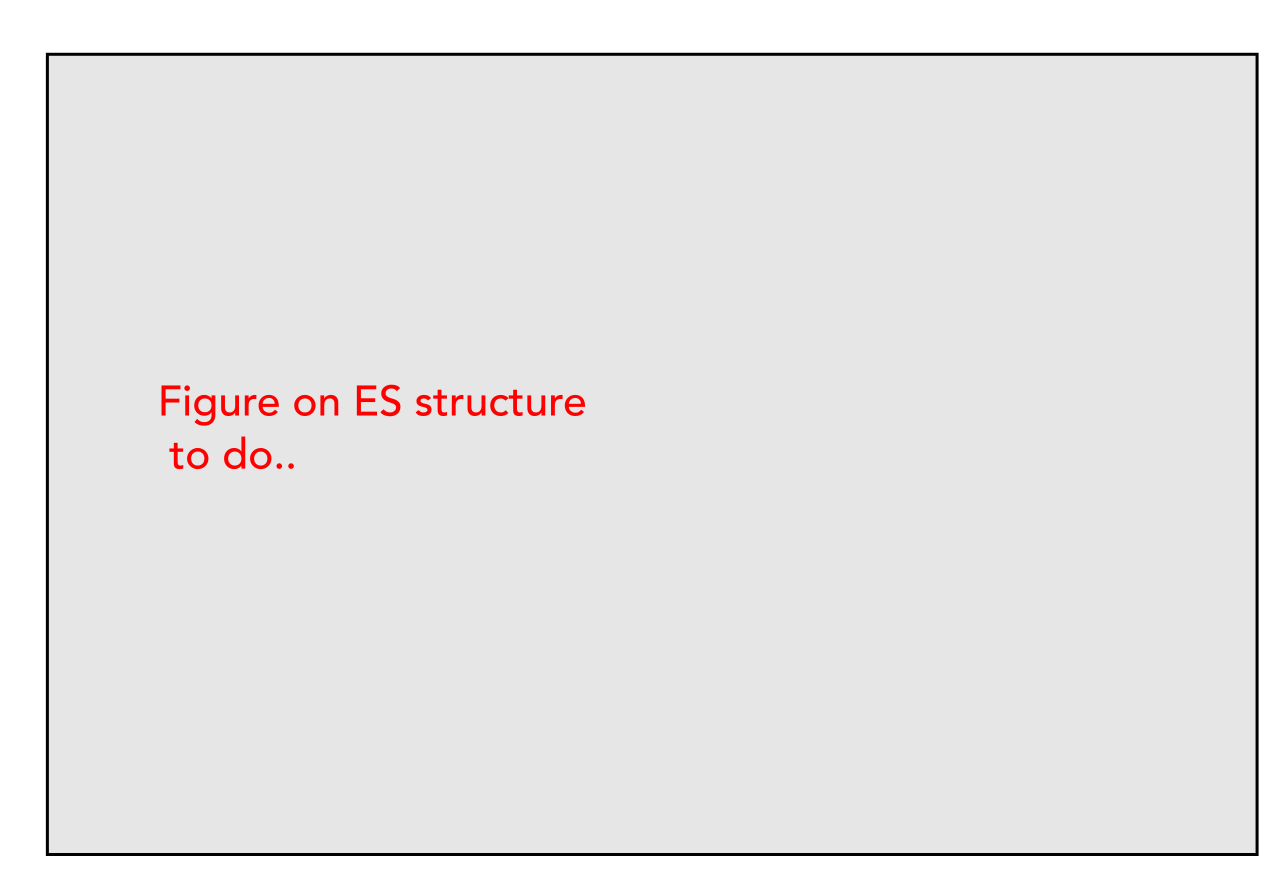
\includegraphics[width=1\linewidth]{Figures/Comparison} 

}

\caption{ES conceptual framework}(\#fig:Fig:ES)
\end{figure}

Efforts on biodiversity conservation relies on the highlight of the economic aspects of biodiversity and the natural capital (\protect\hyperlink{ref-Costanza1997}{Costanza et al. 1997}) and the environmental inaction related to the cost of policy damage occurring in the absence of an effective regulatory framework (\protect\hyperlink{ref-Bruel2016}{Bruel et al. 2016}).
From a strong sustainability perspective, a declining capital stock is an unambiguous indicator of unsustainability in the flow of goods and services that derive from it (\protect\hyperlink{ref-Ekins2003}{Ekins et al. 2003}).
More important, the recognition of the non-substitutability of natural capital with regard to the other forms of capital; acknowledging the characteristics of irreversibility (such as species extinction or climate change), uncertainty and the existence of \emph{critical} components that make a major contribution to welfare.
The main core of the environmental problem relies on the use of use ecosystem's functions, mainly those that generate economic welfare, that are making a negative impact and influence on the natural capital stock, and even worse, on those functions that are responsible for ecosystem stability and resilience (\protect\hyperlink{ref-Ekins2003}{Ekins et al. 2003}).

The Common International Classification of Ecosystem Services (CICES) was developed to provide hiecharchally consistent and science-based classification to be used for natural capital accounting purposes (\protect\hyperlink{ref-ref}{\textbf{ref?}}).
In CICES framework, \protect\hyperlink{ref-Potschin-Young2018}{Potschin-Young et al.} (\protect\hyperlink{ref-Potschin-Young2018}{2018}) argued the conceptual framework of cascading aspect from ecosystesm service are commonly divided Groups, division.

\begin{figure}[!ht]

{\centering 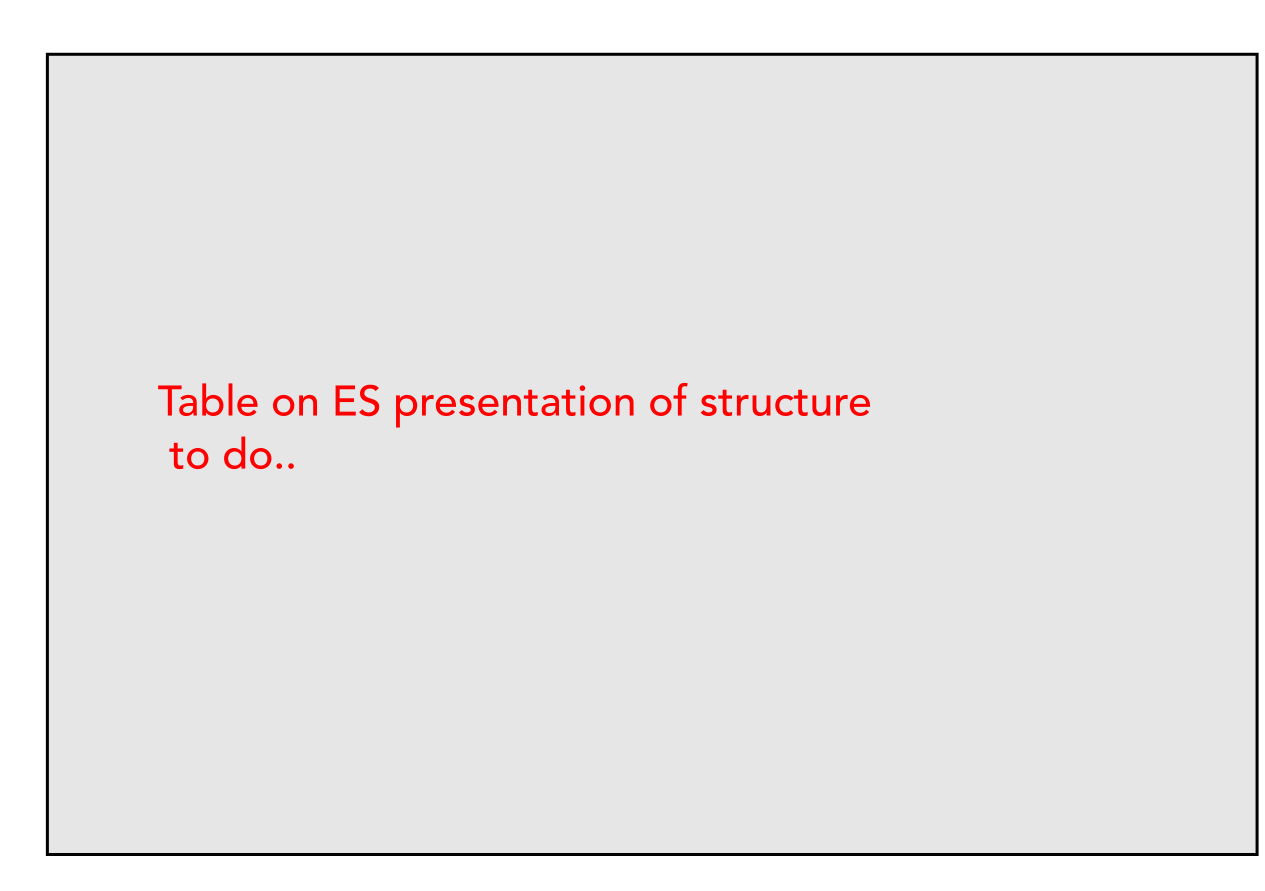
\includegraphics[width=1\linewidth]{Figures/cices} 

}

\caption{ES conceptual framework}\label{fig:Fig-ES-cices}
\end{figure}

The CICES scheme, on the other hand, refers to ES specifically as the products from ecosystem, which can be directly used by human-beings {[}70{]}.
With this definition, supporting services defined in MEA scheme are excluded from CICES scheme, because supporting services cannot be directly consumed by human beings.
The product-based CICES framework can enable clearer mapping between ecological and economic products.
The hierarchical structure of CICES scheme has provisioning, regulating and cultural services at the highest (section) level.
The following levels organize ES according to their divisions, groups and classes.
At lower levels, more specific services can be defined and characterized.
For example, at section level, we may have only the provisioning service but at class level, we may define the service to be forage grass cultivated as animal feed.
Therefore, the hierarchical structure can supply different levels of detail needed by decision makers.

Figure 2.2 demonstrates the hierarchical structure of CICES scheme.

\hypertarget{methodology}{%
\section{Methodology}\label{methodology}}

The purpose of this article is to evaluate the supply and demand of eecosystem services for a prospective distributed recycling chain for additive manufacturing.
A conceptual framework to evaluate the synergy of prospective industrial filières considering the technological and ecological spheres.

\begin{figure}[!ht]

{\centering 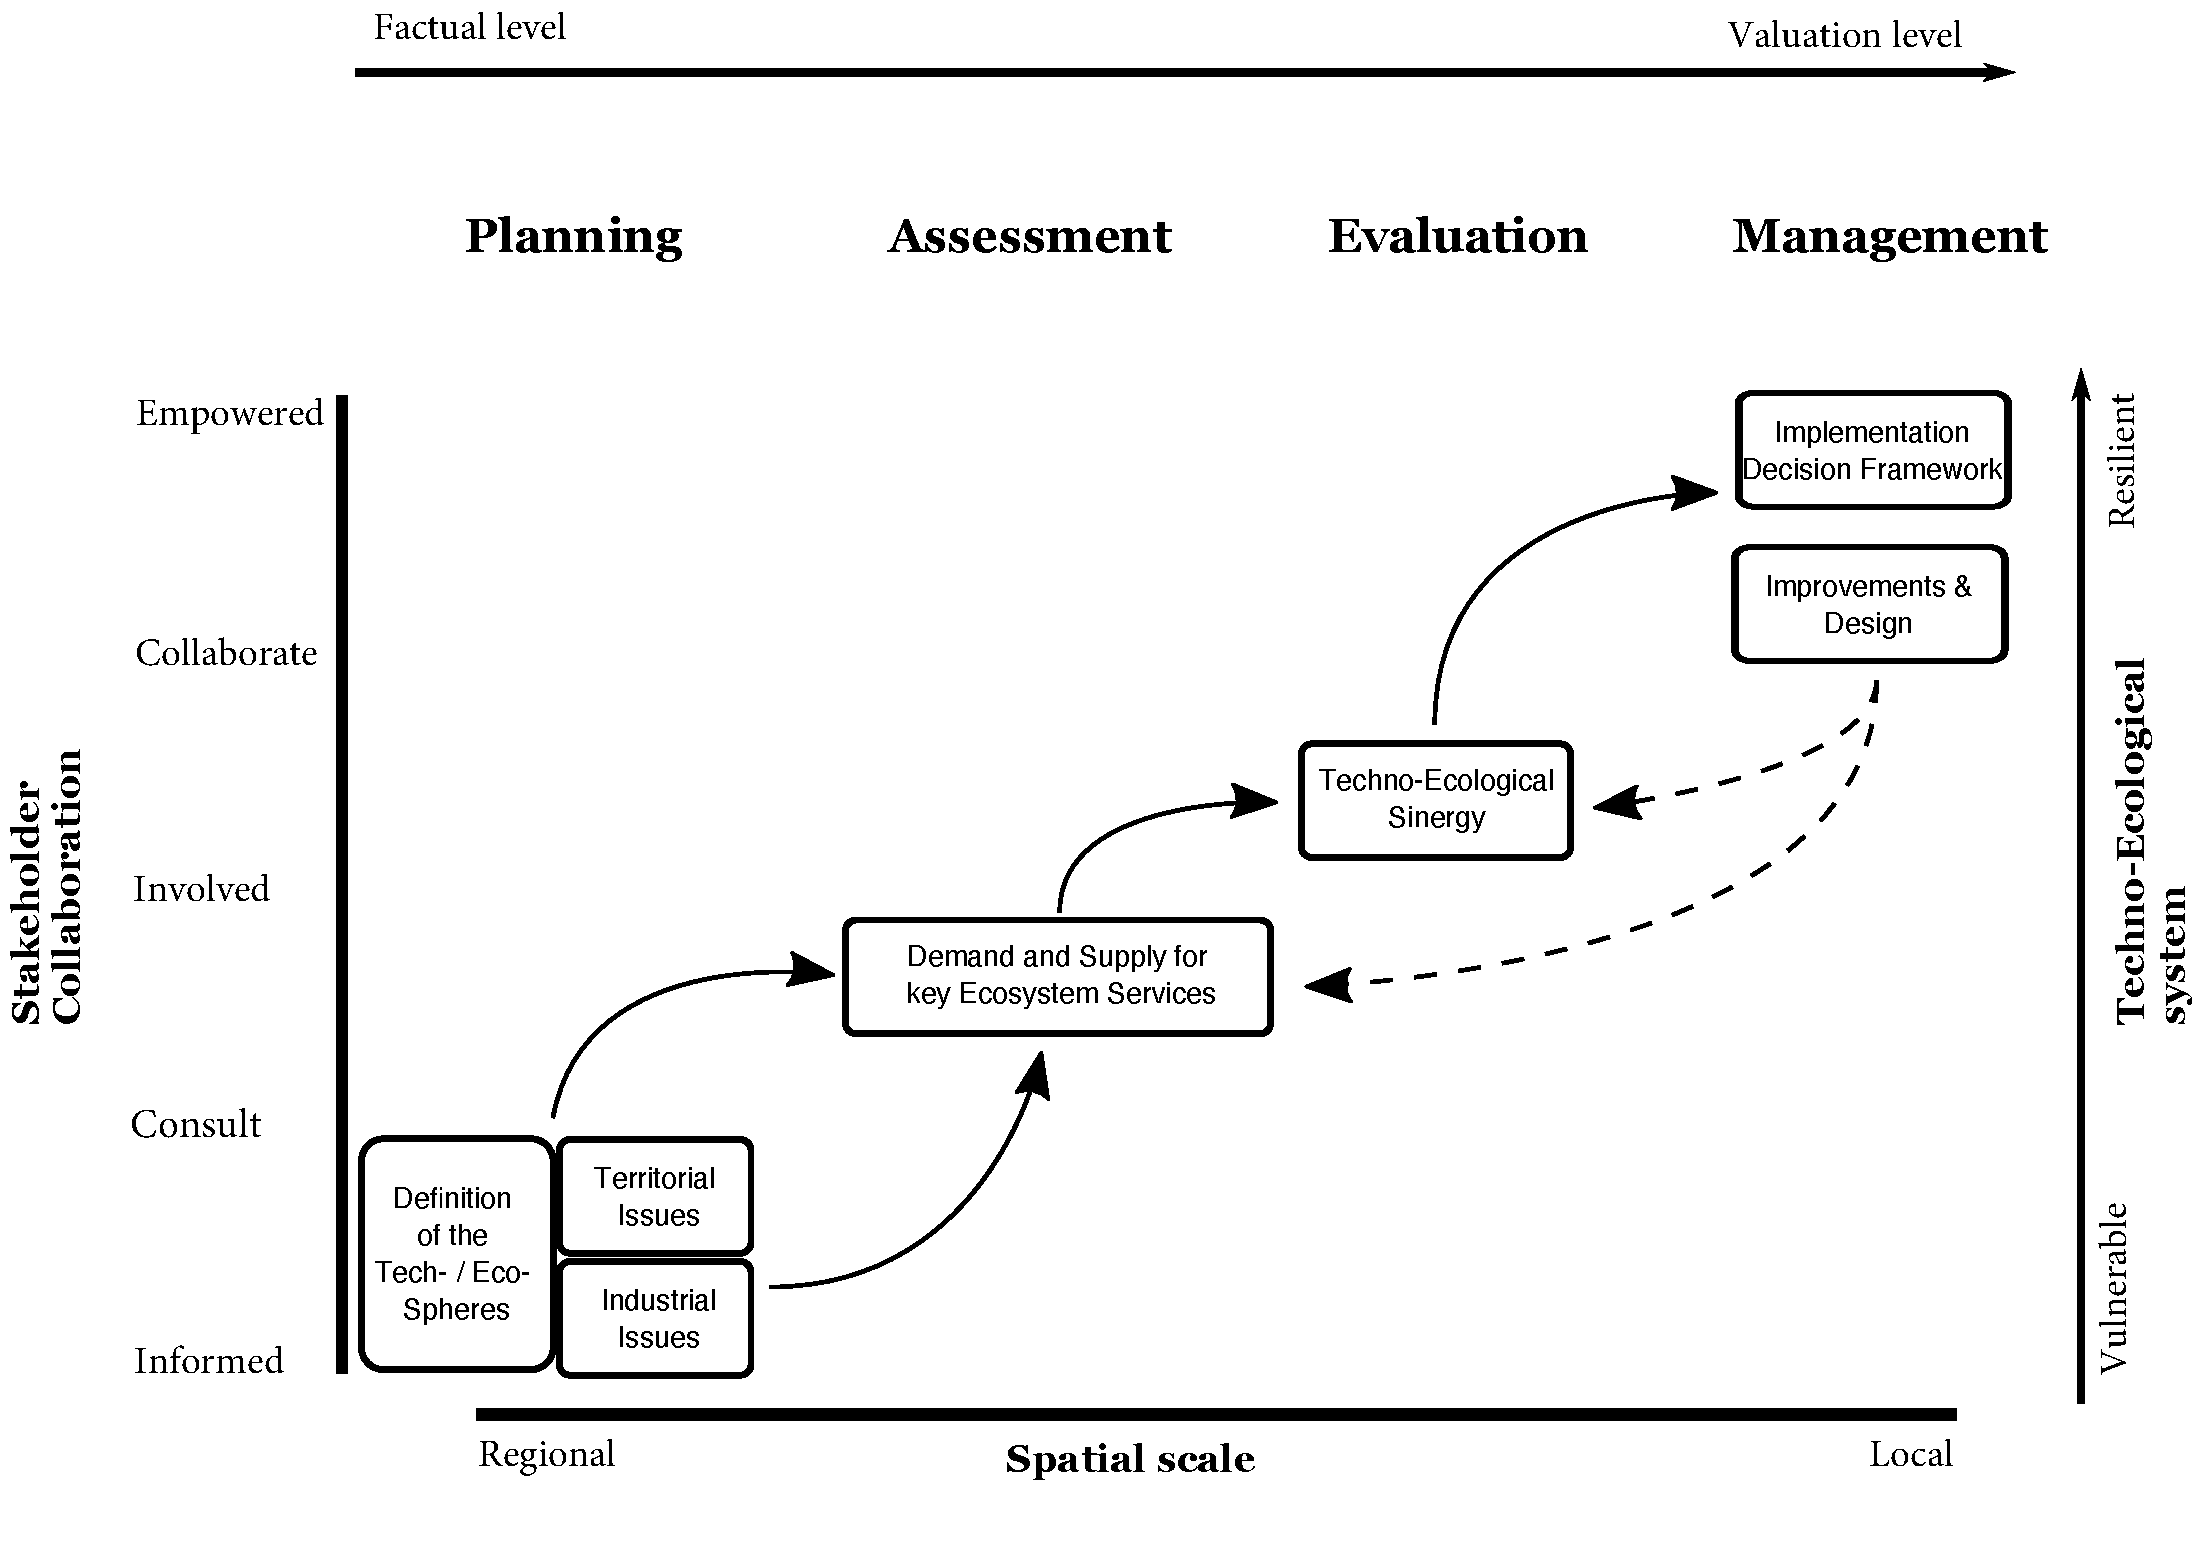
\includegraphics[width=1\linewidth]{Figures/Methodology} 

}

\caption{Operational framework for evaluatig the ecosystem services of industrial systems}\label{fig:Fig-Methodology}
\end{figure}

Four major steps are proposed as illustrated in figure \ref{Fig-Methodology} .

The goal of \emph{Planning} step is to identify the boundaries for the technological and ecological systems to be evaluated.
In the \emph{Assessment} step, the main aim is to jeopardize the key ecosystems services and the respective scales that are going to be included in the analysis.
These elements will be a intersection of the technological and geographical issues based on a analysis of each systems.
In the \emph{Evaluation} stage, the main purpose is to establish the demand and supply of ES based on respective inventory and models. This include the specific allocation
Finally, in the last step \emph{Management}, the main goal is to establish scenarios of evaluation based on the `Bussiness-as-usual' and Synergy frameworks.
This will enable to take a more informed decision to stakeholder at the evaluation of prospopective projects.

An application of the framework will be presented in Section XX using as case study of the distributed recycling chain via additive manufacturing..
In the following sub-sections, each stage of the methodology is explained.

\hypertarget{results}{%
\section{Results}\label{results}}

\hypertarget{step-i---definition-the-industrial-system-distributed-recycling-via-additive-manufacturing}{%
\subsection{Step I - Definition the Industrial system : Distributed recycling via additive manufacturing}\label{step-i---definition-the-industrial-system-distributed-recycling-via-additive-manufacturing}}

Major technological advance in the Additive manufacturing field have enable the validation of distributed fabrication.
In the same logic, recently, the concept of distributed recycling via additive manufacturing (DRAM) emerged in the literature to face the socio-environmental challenges related to recycling option for AM technologies using plastic material as feedstock (\protect\hyperlink{ref-CruzSanchez2020}{Cruz Sanchez et al. 2020}; \protect\hyperlink{ref-Santander2020}{Santander et al. 2020}).

The main hypothesis relies on the fact that a distributed and local spaces can provide recycled feedstock to transform it into finish (or prototypes) for a local community.
To do so, the use of additive manufacturing enables the technical paths to achieve this objective.
While not all types of materials can be recycled given the technical difficulties, the estimation of the environmental advantage is needed to assess at early stages the pertinence of this distributed approaches.
However, as with any recycling system, its feasibility and real impact must be evaluated before its implementation.
Although research has been conducted regarding on the technical and logistical feasibility of distributed plastic recycling, little is known about its pertinence from the ecosystem services perspective in a territory.

The system depicted is presented in the figure XX.
The ES-LCIA framework proposed by was applied to the version of life cycle analysis of distributed recycling develped by .
Because Es are expected to be more relevant in the

The goal of this study is to evaluate and compare the change in ES provisioning
The functional unit (FU) is represented by \emph{1kg of recycled filament delivered at school}.

\hypertarget{step-ii---ecosystem-services-priorities-at-the-territorial-level-nancy-france}{%
\subsection{Step II - Ecosystem services Priorities at the territorial level: Nancy, France}\label{step-ii---ecosystem-services-priorities-at-the-territorial-level-nancy-france}}

Three main elements needs to be carry out in this phase: 1) definition of the technological and ecological spheres, 2) prioritization of the territorial issues, and 3) identification of the industrial issues.

\hypertarget{step-iii---ecosystem-services-issues-at-the-value-chain-plastic-issues-at-the-ecosystems}{%
\subsection{Step III - Ecosystem Services issues at the Value chain: Plastic issues at the ecosystems}\label{step-iii---ecosystem-services-issues-at-the-value-chain-plastic-issues-at-the-ecosystems}}

\hypertarget{step-ii---identifying-the-hot-spot-of-the}{%
\subsection{Step II - Identifying the Hot spot of the}\label{step-ii---identifying-the-hot-spot-of-the}}

\hypertarget{discussion-and-perspective-of-the-analysis}{%
\section{Discussion and perspective of the analysis}\label{discussion-and-perspective-of-the-analysis}}

\hypertarget{conclusions}{%
\section{Conclusions}\label{conclusions}}

\newpage

\hypertarget{references}{%
\section*{References}\label{references}}
\addcontentsline{toc}{section}{References}

\hypertarget{refs}{}
\begin{CSLReferences}{1}{0}
\leavevmode\hypertarget{ref-Bakshi2018}{}%
Bakshi, Bhavik R, Timothy G Gutowski, and Dusan P Sekulic. 2018. {``{Claiming Sustainability: Requirements and Challenges}.''} \emph{ACS Sustain. Chem. Eng.} 6 (3): 3632--39. \url{https://doi.org/10.1021/acssuschemeng.7b03953}.

\leavevmode\hypertarget{ref-Bakshi2015}{}%
Bakshi, Bhavik R, Guy Ziv, and Michael D Lepech. 2015. {``{Techno-Ecological Synergy: A Framework for Sustainable Engineering}.''} \emph{Environ. Sci. Technol.} 49 (3): 1752--60. \url{https://doi.org/10.1021/es5041442}.

\leavevmode\hypertarget{ref-Bruel2018}{}%
Bruel, Aurélien, Jakub Kronenberg, Nadège Troussier, and Bertrand Guillaume. 2019. {``{Linking Industrial Ecology and Ecological Economics: A Theoretical and Empirical Foundation for the Circular Economy}.''} \emph{J. Ind. Ecol.} 23 (1): 12--21. \url{https://doi.org/10.1111/jiec.12745}.

\leavevmode\hypertarget{ref-Bruel2016}{}%
Bruel, Aurélien, Nadège Troussier, Bertrand Guillaume, and Natalia Sirina. 2016. {``{Considering Ecosystem Services in Life Cycle Assessment to Evaluate Environmental Externalities}.''} \emph{Procedia CIRP} 48: 382--87. \url{https://doi.org/10.1016/j.procir.2016.03.143}.

\leavevmode\hypertarget{ref-Ceschin2016}{}%
Ceschin, Fabrizio, and Idil Gaziulusoy. 2016. {``{Evolution of design for sustainability: From product design to design for system innovations and transitions}.''} \emph{Des. Stud.} 47 (November): 118--63. \url{https://doi.org/10.1016/j.destud.2016.09.002}.

\leavevmode\hypertarget{ref-Costanza1997}{}%
Costanza, Robert, Ralph D'Arge, Rudolf de Groot, Stephen Farber, Monica Grasso, Bruce Hannon, Karin Limburg, et al. 1997. {``{The value of the world's ecosystem services and natural capital}.''} \emph{Nature} 387 (6630): 253--60. \url{https://doi.org/10.1038/387253a0}.

\leavevmode\hypertarget{ref-Costanza2017}{}%
Costanza, Robert, Rudolf de Groot, Leon Braat, Ida Kubiszewski, Lorenzo Fioramonti, Paul Sutton, Steve Farber, and Monica Grasso. 2017. {``{Twenty years of ecosystem services: How far have we come and how far do we still need to go?}''} Elsevier B.V. \url{https://doi.org/10.1016/j.ecoser.2017.09.008}.

\leavevmode\hypertarget{ref-CruzSanchez2020}{}%
Cruz Sanchez, Fabio A., Hakim Boudaoud, Mauricio Camargo, and Joshua M. Pearce. 2020. {``{Plastic recycling in additive manufacturing: A systematic literature review and opportunities for the circular economy}.''} \emph{J. Clean. Prod.} 264 (August): 121602. \url{https://doi.org/10.1016/j.jclepro.2020.121602}.

\leavevmode\hypertarget{ref-DeGroot2002}{}%
De Groot, Rudolf S., Matthew A. Wilson, and Roelof M. J. Boumans. 2002. {``{A typology for the classification, description and valuation of ecosystem functions, goods and services}.''} \emph{Ecol. Econ.} 41 (3): 393--408. \url{https://doi.org/10.1016/S0921-8009(02)00089-7}.

\leavevmode\hypertarget{ref-Diwekar2021}{}%
Diwekar, U., A. Amekudzi-Kennedy, B. Bakshi, R. Baumgartner, R. Boumans, P. Burger, H. Cabezas, et al. 2021. {``{A perspective on the role of uncertainty in sustainability science and engineering}.''} \emph{Resour. Conserv. Recycl.} 164 (January): 105140. \url{https://doi.org/10.1016/j.resconrec.2020.105140}.

\leavevmode\hypertarget{ref-Ekins2003}{}%
Ekins, Paul, Sandrine Simon, Lisa Deutsch, Carl Folke, and Rudolf De Groot. 2003. {``{A framework for the practical application of the concepts of critical natural capital and strong sustainability}.''} \emph{Ecol. Econ.} 44 (2-3): 165--85. \url{https://doi.org/10.1016/S0921-8009(02)00272-0}.

\leavevmode\hypertarget{ref-Gopalakrishnan2016}{}%
Gopalakrishnan, Varsha, Bhavik R. Bakshi, and Guy Ziv. 2016. {``{Assessing the capacity of local ecosystems to meet industrial demand for ecosystem services}.''} \emph{AIChE J.} 62 (9): 3319--33. \url{https://aiche.onlinelibrary.wiley.com/doi/full/10.1002/aic.15340\%20https://aiche.onlinelibrary.wiley.com/doi/abs/10.1002/aic.15340\%20https://aiche.onlinelibrary.wiley.com/doi/10.1002/aic.15340}.

\leavevmode\hypertarget{ref-Gomez-Baggethun2010}{}%
Gómez-Baggethun, Erik, Rudolf de Groot, Pedro L. Lomas, and Carlos Montes. 2010. {``{The history of ecosystem services in economic theory and practice: From early notions to markets and payment schemes}.''} \emph{Ecol. Econ.} 69 (6): 1209--18. \url{https://doi.org/10.1016/j.ecolecon.2009.11.007}.

\leavevmode\hypertarget{ref-DeGroot2012}{}%
Groot, Rudolf de, Luke Brander, Sander van der Ploeg, Robert Costanza, Florence Bernard, Leon Braat, Mike Christie, et al. 2012. {``{Global estimates of the value of ecosystems and their services in monetary units}.''} \emph{Ecosyst. Serv.} 1 (1): 50--61. \url{https://doi.org/10.1016/j.ecoser.2012.07.005}.

\leavevmode\hypertarget{ref-Harrison2018}{}%
Harrison, Paula A., Rob Dunford, David N. Barton, Eszter Kelemen, Berta Martín-López, Lisa Norton, Mette Termansen, et al. 2018. {``{Selecting methods for ecosystem service assessment: A decision tree approach}.''} \emph{Ecosyst. Serv.} 29 (February): 481--98. \url{https://doi.org/10.1016/j.ecoser.2017.09.016}.

\leavevmode\hypertarget{ref-Honeck2021}{}%
Honeck, Erica, Louise Gallagher, Bertrand von Arx, Anthony Lehmann, Nicolas Wyler, Olga Villarrubia, Benjamin Guinaudeau, and Martin A. Schlaepfer. 2021. {``{Integrating ecosystem services into policymaking -- A case study on the use of boundary organizations}.''} \emph{Ecosyst. Serv.} 49 (June): 101286. \url{https://doi.org/10.1016/j.ecoser.2021.101286}.

\leavevmode\hypertarget{ref-Kumar2021}{}%
Kumar, Rakesh, Anurag Verma, Arkajyoti Shome, Rama Sinha, Srishti Sinha, Prakash Kumar Jha, Ritesh Kumar, et al. 2021. {``{Impacts of Plastic Pollution on Ecosystem Services, Sustainable Development Goals, and Need to Focus on Circular Economy and Policy Interventions}.''} \emph{Sustainability} 13 (17): 9963. \url{https://doi.org/10.3390/su13179963}.

\leavevmode\hypertarget{ref-Laurans2013}{}%
Laurans, Yann, Aleksandar Rankovic, Raphaël Billé, Romain Pirard, and Laurent Mermet. 2013. {``{Use of ecosystem services economic valuation for decision making: Questioning a literature blindspot}.''} Academic Press. \url{https://doi.org/10.1016/j.jenvman.2013.01.008}.

\leavevmode\hypertarget{ref-Liu2019g}{}%
Liu, Xinyu, and Bhavik R. Bakshi. 2019. {``{Ecosystem Services in Life Cycle Assessment while Encouraging Techno‐Ecological Synergies}.''} \emph{J. Ind. Ecol.} 23 (2): 347--60. \url{https://doi.org/10.1111/jiec.12755}.

\leavevmode\hypertarget{ref-Lomborg2020}{}%
Lomborg, Bjorn. 2020. {``{Welfare in the 21st century: Increasing development, reducing inequality, the impact of climate change, and the cost of climate policies}.''} \emph{Technol. Forecast. Soc. Change} 156 (July): 119981. \url{https://doi.org/10.1016/j.techfore.2020.119981}.

\leavevmode\hypertarget{ref-Mahmud2021}{}%
Mahmud, Roksana, Sheikh Moniruzzaman Moni, Karen High, and Michael Carbajales-Dale. 2021. {``{Integration of techno-economic analysis and life cycle assessment for sustainable process design -- A review}.''} Elsevier. \url{https://doi.org/10.1016/j.jclepro.2021.128247}.

\leavevmode\hypertarget{ref-Martinez-Hernandez2017}{}%
Martinez-Hernandez, Elias. 2017. {``{Trends in sustainable process design---from molecular to global scales}.''} \emph{Curr. Opin. Chem. Eng.} 17 (August): 35--41. \url{https://doi.org/10.1016/j.coche.2017.05.005}.

\leavevmode\hypertarget{ref-MEA2005}{}%
MEA. 2005. {``{Ecosystems and Human well-being: Synthesis}.''} \href{https://www.islandpress.org}{www.islandpress.org}.

\leavevmode\hypertarget{ref-ONeill2018}{}%
O'Neill, Daniel W., Andrew L. Fanning, William F. Lamb, and Julia K. Steinberger. 2018. {``{A good life for all within planetary boundaries}.''} \emph{Nat. Sustain.} 1 (2): 88--95. \url{https://doi.org/10.1038/s41893-018-0021-4}.

\leavevmode\hypertarget{ref-PedersenZari2019}{}%
Pedersen Zari, Maibritt. 2019. {``{Ecosystem services impacts as part of building materials selection criteria}.''} \emph{Mater. Today Sustain.} 3-4. \url{https://doi.org/10.1016/j.mtsust.2019.100010}.

\leavevmode\hypertarget{ref-Potschin-Young2018}{}%
Potschin-Young, M., R. Haines-Young, C. Görg, U. Heink, K. Jax, and C. Schleyer. 2018. {``{Understanding the role of conceptual frameworks: Reading the ecosystem service cascade}.''} \emph{Ecosyst. Serv.} 29 (February): 428--40. \url{https://doi.org/10.1016/j.ecoser.2017.05.015}.

\leavevmode\hypertarget{ref-Pryshlakivsky2021}{}%
Pryshlakivsky, Jonathan, and Cory Searcy. 2021. {``{Life Cycle Assessment as a decision-making tool: Practitioner and managerial considerations}.''} Elsevier. \url{https://doi.org/10.1016/j.jclepro.2021.127344}.

\leavevmode\hypertarget{ref-Rockstrom2009}{}%
Rockström, Johan, Will Steffen, Kevin Noone, Åsa Persson, F. Stuart Chapin, Eric F. Lambin, Timothy M. Lenton, et al. 2009. {``{A safe operating space for humanity}.''} \url{https://doi.org/10.1038/461472a}.

\leavevmode\hypertarget{ref-Rodrigues2021}{}%
Rodrigues, Jérémy, Natacha Gondran, Adrien Beziat, and Valérie Laforest. 2021. {``{Application of the absolute environmental sustainability assessment framework to multifunctional systems -- The case of municipal solid waste management}.''} \emph{J. Clean. Prod.} 322: 129034. \url{https://doi.org/10.1016/j.jclepro.2021.129034}.

\leavevmode\hypertarget{ref-RoyHaines-Young2018}{}%
Roy Haines-Young, by, and Marion Potschin. 2018. {``{Common International Classification of Ecosystem Services (CICES) V5.1 Guidance on the Application of the Revised Structure}.''} \href{https://www.cices.eu}{www.cices.eu}.

\leavevmode\hypertarget{ref-Santander2020}{}%
Santander, Pavlo, Fabio A Cruz Sanchez, Hakim Boudaoud, and Mauricio Camargo. 2020. {``{Closed loop supply chain network for local and distributed plastic recycling for 3D printing: a MILP-based optimization approach}.''} \emph{Resour. Conserv. Recycl.} 154 (March): 104531. \url{https://doi.org/10.1016/j.resconrec.2019.104531}.

\leavevmode\hypertarget{ref-TEEB2010}{}%
TEEB. 2010. \emph{{The Economics of Ecosystems and Biodiversity Ecological and Economic Foundations.}} \url{https://doi.org/10.4324/9781849775489}.

\leavevmode\hypertarget{ref-Torres2021}{}%
Torres, Angélica Valencia, Chetan Tiwari, and Samuel F. Atkinson. 2021. {``{Progress in ecosystem services research: A guide for scholars and practitioners}.''} \emph{Ecosyst. Serv.} 49 (June): 101267. \url{https://doi.org/10.1016/j.ecoser.2021.101267}.

\leavevmode\hypertarget{ref-Wallner1996}{}%
Wallner, H. P., M. Narodoslawsky, and F. Moser. 1996. {``{Islands of sustainability: A bottom-up approach towards sustainable development}.''} \emph{Environ. Plan. A} 28 (10): 1763--78. \url{https://doi.org/10.1068/a281763}.

\end{CSLReferences}

\end{document}
